\section{场景及假设}
\label{sec:featurespy-setting}

本文提出\sysnameF 通过在客户端可信执行环境中通过主动检测推测内容攻击来增强加密重复数据删除,从而完全击败依赖侧信道信息的恶意客户端。

\paragraph*{部署场景。}图~\ref{fig:featurespy-model}展示将\sysnameF 部署在加密重复数据删除的方式。为了部署\sysnameF,本文首先将安全区代码编译成动态链接库\citing{sgx},并将动态链接库连同用于完整性验证的签名分发给每个客户端。云服务端托管动态链接库以验证每个客户端的安全区。具体来说,客户端初始化\sysnameF,通过加载动态链接库创建对应的安全区,云服务端通过远程证明\citing{sgx}(参见\S\ref{subsec:background-tee-sgx})对每个安全区进行认证,以确保将正确的代码加载到安全区中。

\begin{figure}[!htb]
    \centering
    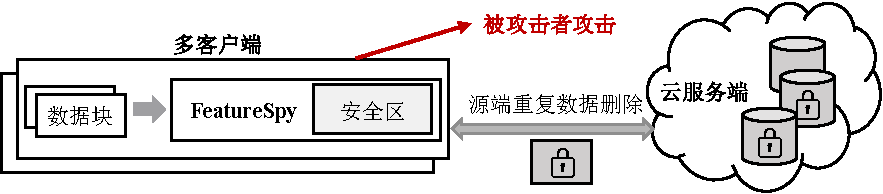
\includegraphics[width=\textwidth]{pic/featurespy/deployment.pdf}
    \caption{部署\sysnameF}
    \label{fig:featurespy-model}
\end{figure}

在数据上传过程中,\sysnameF 处理明文数据块(由客户端生成),并为源端重复数据删除计算相应的密文数据块和指纹。正常的客户端仅将不重复的密文数据块传输到云服务端。当\sysnameF 检测到客户端可能被攻击并正在发起推测内容攻击,则向云服务端报告该恶意客户端以停止云服务端对该客户端的响应。

\paragraph*{威胁模型。}本文的主要安全目标是增强加密重复数据删除(\S\ref{sec:background-enc-deduplication})以防止恶意客户端发动推测内容攻击。与传统加密重复数据删除\citing{bellare2013MLE}类似,本文考虑了一个旨在从任何存储的密文数据块中窃取原始明文内容的不可信云服务端。此外,本文防御的恶意客户端旨在学习其他正常的客户端的原始明文数据块。具体来说,恶意客户端可以访问其泄露的明文数据块和密钥,并任意伪造新的明文数据块以发起推测内容攻击(\S\ref{sec:featurespy-attack})。此外,它可以篡改未受保护的内存中的内容和操作,以逃避\sysnameF 的检查。


\paragraph*{安全假设。}针对本文的威胁模型,做出以下安全假设:
\begin{itemize}[leftmargin=0em]
    \item 每个客户端与云服务端之间的通信受SSL/TLS保护以防止第三方窃听。
    \item 安全区是受信任且经过身份验证的(例如,在首次启动时通过远程证明验证其可靠性),以便诚实地执行攻击检测并防止检测机制被篡改。此外,现有的基于TEE的加密重复数据删除\citing{shinde20}及\sysnameS 一样,安全区维护密钥(即\S\ref{sec:featurespy-implementation}中的PoW密钥)而不是所有安全区内的机密性,以缩小可信计算基TCB的大小,尽可能降低针对安全区的侧信道攻击产生的风险\citing{fei21}。
    \item 不可信的云服务端可能会破坏外包数据,损害用户数据的完整性。\sysnameF 没有解决该威胁,但它与\gls{pdp}\citing{ateniese2007provable}和\gls{por}\citing{juels2007pors}兼容,可通过执行定期的完整性验证外包数据应对云服务端破坏数据完整性的威胁。\sysnameF 也可与\citing{li15}中的高容错存储结合,以提高数据存储的可靠性。
\end{itemize}